% Options here are passed to the article class.
% Most common options: 10pt, 11pt, 12pt
\documentclass[10pt]{datasheet}

% Input encoding and typographical rules for English language
\usepackage[utf8]{inputenc}
\usepackage[english]{babel}
\usepackage[english]{isodate}

% tikz is used to draw images in this example, but you can
% also use \includegraphics{}.
\usepackage{graphicx}

% These define global texts that are used in headers and titles.
\title{DS01: Streamable Bit RAM}
\author{Andrews54757}
\tags{data-storage, RAM, streamable, binary}
\date{October 2022}
\revision{Revision 1}

\begin{document}
\maketitle

\section{Features}

\begin{itemize}
\item{Constant time writes to individually addressible bits.}
\item{RAM contents can be streamed at a certain rate.}
\item{Matrix decoding addresses memory modules individually to reduce lag.}
\end{itemize}

\section{Applications}

\begin{itemize}
\item{Storing boolean flags for use in streamed logic.}
\item{Reducing unecessary bulk calls in restock systems.}
\end{itemize}

\section{General Description}
The DS01 is a RAM module that stores 1600 bits of data in locked repeaters. Each bit is addressable through three 4-bit inputs. It is able to stream all of its stored data such that one bit is outputted per level every 4gt-8gt.

% Switch to next column
\vfill\break

\begin{figure}[h]
    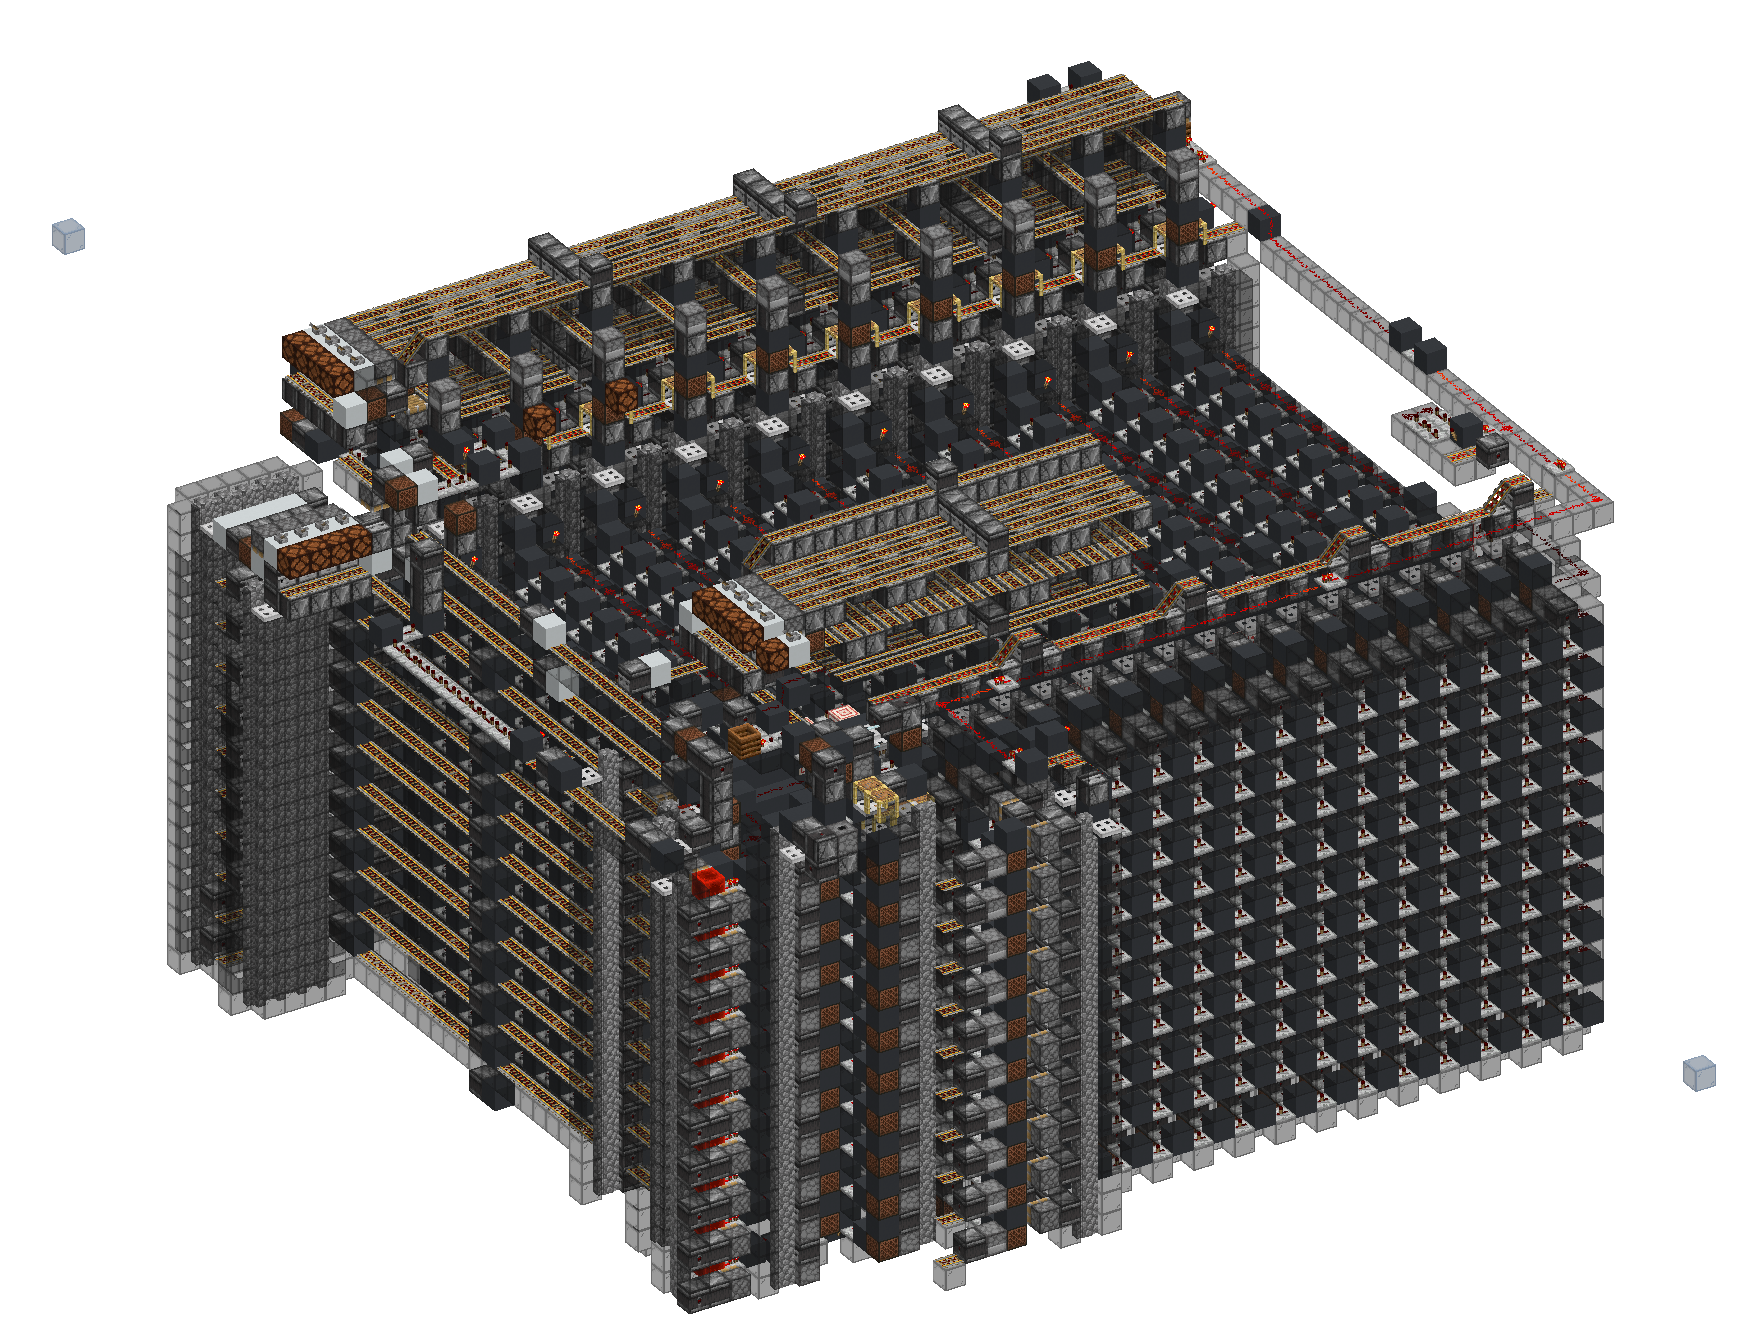
\includegraphics[width=0.45\textwidth]{sram.png}
    \caption{1600 Bit Streamable RAM}
\end{figure}

% For wide tables, a single column layout is better. It can be switched
% page-by-page.
\onecolumn

\section{Device Specifications}

The specifications below are for the 1600 bit variant.

\begin{table}[h]
    \caption{Inputs}
    \begin{tabularx}{\textwidth}{l | c | X}
        \thickhline
        \textbf{Name} & \textbf{Range} & \textbf{Description} \\
        \hline
        Binary Code 1 & 0-9 & First code indicating horizontal section. \\
        Binary Code 2 & 0-9 & Second code indicating vertical position. \\
        Binary Code 3 & 0-15 & Third code indicating repeater location within storage module. \\
        \hline
        Bit Value & 0-1 & Indicates value to write to bit\\
        \hline
        Write bit & Pulse & Writes to a bit \\
        Stream values & Pulse & Streams values as pulsed signals. \\
        \thickhline
\end{tabularx}
\end{table}

\begin{table}[h]
    \caption{Outputs}
    \begin{tabularx}{\textwidth}{l | c | X}
        \thickhline
        \textbf{Name} & \textbf{Range} & \textbf{Description} \\
        \hline
        Streamed values & Pulse & 4-8gt pulses. \\
        \thickhline
\end{tabularx}
\end{table}

\begin{table}[h]
    \caption{Device Specifications}
    \begin{tabularx}{\textwidth}{l | c c c | c | X}
        \thickhline
        \textbf{Parameter} & \textbf{Min.} & \textbf{Typ.} & \textbf{Max.} &
        \textbf{Unit} & \textbf{Conditions} \\
        \hline
        Write Throughput  & 120 & - & - & gt & \multirow{2}{*}{Normal Usage} \\
        Output Throughput Per Level & 4 & - & 8 & gt & \\
        \hline
        Write Active Lag & +0.2 & +0.5 & +1.0 & ms & \multirow{2}{5cm}{Ryzen 5 3600, 2GB RAM. MC 1.18.1 with Lithium.} \\
        Stream Active Lag & +1 & +3 & +5 & ms & \\
        \hline
        MC Version & 1.16 & 1.17.1 & - & MCV & Latest version at time of writing: 1.19.2\\
        \hline
        Dimensions & & 50 x 32 x 50 & & Blocks & \\
        \thickhline
\end{tabularx}
\end{table}
\newpage
\section{Testing Data}
\begin{table}[h]
\caption{Executed Tests}
\begin{tabularx}{\textwidth}{l | X}
    \thickhline
    \textbf{Test} & \textbf{Result} \\
    \hline
    Write test & Device was able to write to all bits successfully.\\
    \hline
    Stream test & Device was able to stream all bits successfully.\\
    \thickhline
\end{tabularx}
\end{table}

\section{Download Information}
\begin{table}[h]
    \caption{Download Information}
    \begin{tabularx}{\textwidth}{l | l | l | X}
        \thickhline
        \textbf{Identifier} & \textbf{MC} & \textbf{File} & \textbf{Description} \\
        \hline
        DS011600 & 1.17.1 & DS011600\_1600\_bit\_RAM\_p1.litematic & Litematic of RAM with 1600 bits. Inventories not included. \\
        \hline
        DS01600 & 1.18.2 & DS01600\_600\_bit\_ram.litematic & Litematic of RAM with 600 bits. Wired slightly better. 36x32x36 blocks. Inventories not included. \\
        \thickhline
    \end{tabularx}
\end{table}

\begin{figure}[h]
    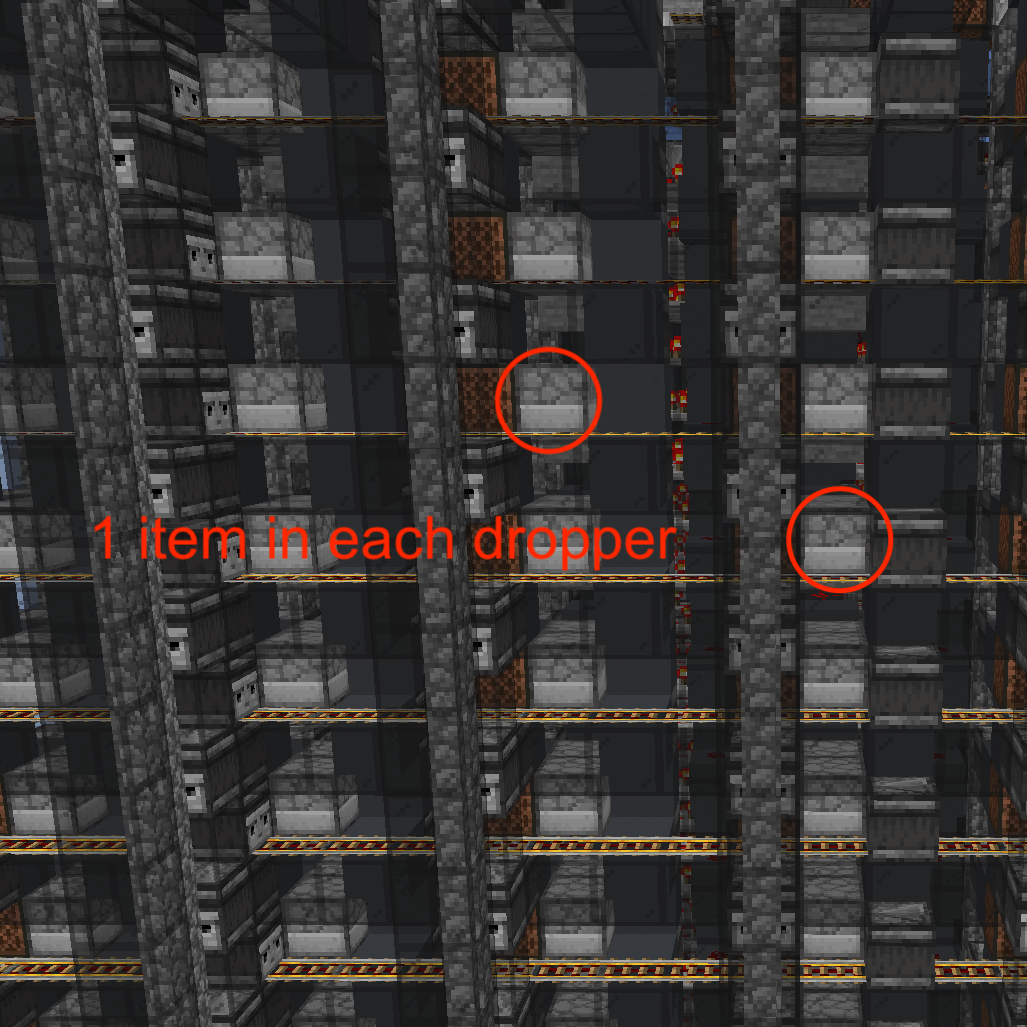
\includegraphics[width=0.45\textwidth]{invs.png}
    \caption{Inventories setup guide}
\end{figure}

\end{document}

